\subsection{QuizziPedia::Back-End::App::Models}
\subsubsection{Informazioni generali}
\label{QuizziPedia::Back-End::App::Models}
\begin{figure}
	\centering
	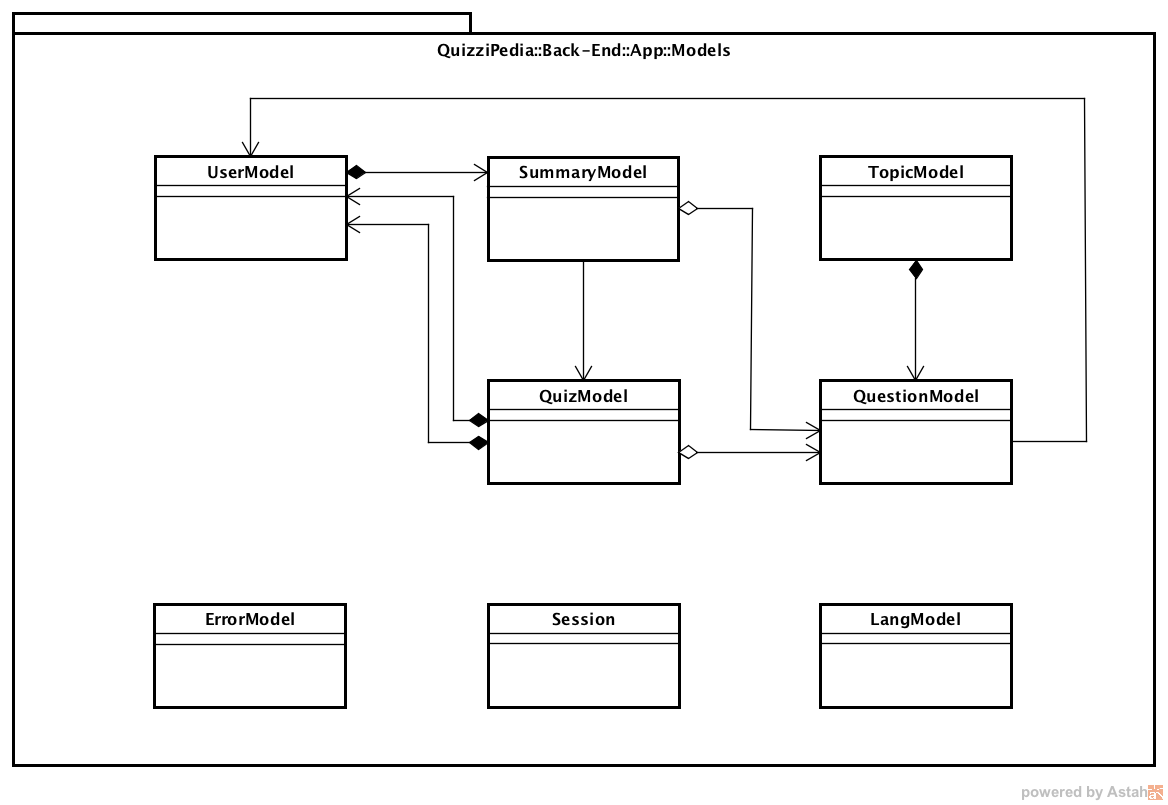
\includegraphics[scale=0.45]{UML/Package/QuizziPedia_Back-End_App_Models.png}
	\caption{QuizziPedia::Back-End::App::Models}
\end{figure}

\subsubsection{Classi}
\paragraph{QuizziPedia::Back-End::App::Models::NOMECLASSE}
\begin{itemize}
	\item \textbf{Descrizione} \\
	\item \textbf{Utilizzo} \\
	\item \textbf{Relazioni con altre classi} \\
	\item \textbf{Metodi} \\
\end{itemize}